\documentclass{sbmlmanual}

\newcommand{\libsbml}{\textsc{libsbml}}

\begin{document}

%=============================================================================
% Title page
%=============================================================================

\title{\libsbml{}\\[5pt]
  Developer's Manual}

\author{Ben Bornstein}

\authoremail{bornstei@cds.caltech.edu}

\address{SBML Team\\
  Control and Dynamical Systems, MC 107-81\\
  California Institute of Technology, Pasadena, CA 91125, USA\\[3pt]
  {\url{http://sbml.org/}}}

\acknowledge{Principal Investigators: John Doyle and Hiroaki Kitano}

\date{DRAFT\\[5pt]
  \today{}}

\maketitlepage




%=============================================================================
\section{Quickstart}
\label{sec:quickstart-unix}
%=============================================================================

\libsbml{} depends on Apache's Xerces-C++ XML library for
low-level XML tokenizing and Unicode support.  Xerces is supported on
Unix (Linux), Windows and MacOS X.  Many popular Linux systems provide
the Xerces library either as part of their standard distribution or as
an optional RPM or Debian package.  Apache provides a Windows binary
distribution which includes both a DLL and a LIB file.  For more
information, see: \url{http://xml.apache.org/xerces-c/}.  The
instructions below assume Apache is already installed on your system.


%-----------------------------------------------------------------------------
\subsection{Linux, Cygwin or MacOS X}
%-----------------------------------------------------------------------------

At the Unix, Cygwin or OS X command prompt, \texttt{untar} the
distribution, \texttt{cd} into the directory created (e.g.,
\texttt{libsbml-1.0.1/}), and type:

\begin{example}[csh]
  % ./configure
  % make
  % make install
\end{example}

To compile programs that use libsbml (e.g., see
Section~\ref{sec:read-example}) with GCC:

\begin{example}[csh]
  % gcc -o myapp.c myapp.c -lsbml
\end{example}


%-----------------------------------------------------------------------------
\subsection{Windows}
%-----------------------------------------------------------------------------

Unzip the distribution and open the resulting folder
(e.g. \texttt{libsbml-1.0.1}).  There are debug (\texttt{libsbmld})
and release (\texttt{libsbml}) versions of \textsc{libsbml}, with
\texttt{.dll} and \texttt{.lib} files for both versions in the
\texttt{Win32} subdirectory.  \textsc{libsbml} header files are
located in \texttt{src/sbml}.

Visual C++ projects should link with \texttt{libsbml.lib} or
\texttt{libsbmld.lib} and generate code for the Multithreaded DLL or
Debug Multithreaded DLL version of the VC++ runtime, respectively.


%=============================================================================
\section{Introduction}
\label{sec:introduction}
%=============================================================================

This manual describes \textsc{libsbml}, a C application programming
interface (API) library for reading, writing and manipulating the Systems
Biology Markup
Language~\citep[SBML;][]{hucka:2001,hucka:2003,finney:2003c}.  Currently,
the library supports SBML Level~1 Version~1 and Version~2, and nearly all
of SBML Level~2 Version~1.  (The still-unimplemented parts of Level~2 are:
support for RDF, and support for MathML's \texttt{semantics},
\texttt{annotation} and \texttt{annotation-xml} elements.  These will be
implemented in the near future.)  For more information about SBML, please
see the references or visit \url{http://www.sbml.org/} on the Internet.

Since the library provides a C API, familiarity with the C programming
language is assumed.  Some parts of the library were written in C++,
however, experience with C++ is not required; its use is ``hidden''
behind C functions.  A companion document~\citep{bornstein:2003b} provides
a detailed reference manual for the API.

\libsbml{} is entirely open-source and all specifications and
source code are freely and publicly available.  For more information
about SBML, please see the references section or visit
\url{http://www.sbml.org/}.

Some of the features of \textsc{libsbml} include:


\begin{itemize}

  \item \textbf{Small Memory Footprint}

  The parser is event-based (SAX2) and loads SBML data into C
  structures that mirror the classes in the SBML specification.  No
  intermediate DOM is used, which greatly reduces runtime memory
  usage.

  \item \textbf{Fast Runtime}

  The Gepasi generated 100 Yeast file (2Mb; 2000 reactions
  \url{http://www.gepasi.org/gep3sbml.html}) loads in 1.18s on a 1 GHz
  AMD Athlon XP and uses 1.4Mb of memory.

  \item \textbf{Portable}

  The C source code is pure ANSI for maximum portability.  It produces
  no errors or warnings when compiled with either GCC or Microsoft
  Visual C++.  GCC compilation flags are: \texttt{-ansi
  -pedantic-errors -Wall}, i.e., ANSI violations are compilation errors
  instead of warnings and all warnings are reported.

  The build system uses the GNU Autotools (Autoconf, Automake, and
  Libtool) to build shared and static libraries on a variety of
  Unix-based platforms.

  Microsoft Windows is supported either through the Cygwin environment
  or as a native Win32 Dynamic Link Library (DLL).  A Microsoft Visual
  C++ 6.0 project file is included in the source distribution and a
  precompiled Windows distribution is available.

  \item \textbf{Full SBML Support}

  The parser supports both spellings of \emph{species} and
  \emph{annotation} (i.e., with and without the last \emph{s}) for any
  level and version.  When writing SBML documents, the appropriate
  specification-sanctioned spelling is used.

  The full-text (including any namespace declarations) of
  \texttt{<notes>} and \texttt{<annotation>} elements may be retrieved
  from any SBML object.  For compatibility with some technically
  incorrect but popular SBML documents, the parser recognizes and
  stores notes and annotations defined for the top-level
  \texttt{<sbml>} element (though a warning is logged).

  \item \textbf{Full XML Schema Validation}

  The library uses the Apache Xerces-C++ XML library, which supports
  full XML Schema validation.  All XML and Schema warning, error and
  fatal error messages are logged with line and column number
  information and may be retrieved and manipulated pragmatically.  The
  Schema file to use for validation is configurable.

  \item \textbf{Full Unicode Support}

  SBML Documents are parsed and manipulated in the Unicode codepage
  for efficiency (this is Xerces-C++ native format); however, strings
  are transcoded to the local code page for the SBML C structures.

  \item \textbf{Well Tested}

  The entire library was written using the test-first approach
  popularized by Kent Beck and eXtreme Programming, where it's one of
  the 12 principles.

  Currently there are 3014 individual assertions in 583 functional
  unit tests.  Four test cases are responsible for reading entire SBML
  files (three are examples from the L1 document) into memory and
  verifying every field of the resulting structures.

  \item \textbf{Conscientious Use of Memory}

  All memory for and contained in SBML structures is C memory, so
  \method{realloc()} and \method{free()} may be used.  This is an
  important distinction when working with mixed C and C++ code.  C's
  \method{malloc()} and \method{free()} are not compatible with C++'s
  \method{new} and \method{delete} operators.

  A custom memory trace facility can be used to track all memory
  allocated and freed in both the library and all test suites.  This
  facility must be enabled at build time with \texttt{./configure
  --enable-memory-tracing}.  For performance reasons memory tracing
  should be turned off in production environments.  Currently all unit
  tests produce 1782 memory allocations and matched frees with no
  leaks.

\end{itemize}


%=============================================================================
\section{Installation}
\label{sec:installation}
%=============================================================================


\libsbml{} depends on Apache's Xerces-C++ XML library for
low-level XML tokenizing and Unicode support.  Xerces is supported on
Unix (Linux), Windows and MacOS X.  Many popular Linux systems provide
the Xerces library either as part of their standard distribution or as
an optional RPM or Debian package.  Apache provides a Windows binary
distribution which includes both a DLL and a LIB file.

For more information, see:

\begin{quote}
  \url{http://xml.apache.org/xerces-c/}
\end{quote}

A good way to determine whether or not Xerces-C is installed is to run
the build script (see below); it will halt if it cannot find the
Xerces-C library.

\libsbml{} is designed to be extremely portable.  It is written
in 100\% pure ANSI-C and the build system uses the GNU Autotools
(Autoconf, Automake and Libtool).  In most cases, building should be
as easy unpacking the sources and running:

\begin{example}[csh]
  % ./configure
  % make
  % make check    (optional)
  % make install
\end{example}

However, if Xerces-C is installed in a non-standard place (e.g., a
home directory), configure will not be able to detect it.  In this
case, configure needs to be told explicitly where to find the library.
Set the \variable{CPPFLAGS} and \variable{LDFLAGS} environment
variables to include the custom directories containing Xerces-C header
and library files.  For example:

\begin{example}[csh]
  % export CPPFLAGS=-I/home/bornstei/software/xerces-c/2.2.0/include
  % export LDFLAGS=-L/home/bornstei/software/xerces-c/2.2.0/lib
  % ./configure
  % # etc.
\end{example}

\texttt{make install} copies header files to
\texttt{/usr/local/include/sbml} and (shared and static) library files
to \texttt{/usr/local/lib}.  To specify a different install location
use:

\begin{example}[csh]
  % ./configure --prefix=/my/favorite/path
\end{example}


\texttt{make check} is optional and will build and run an extensive
suite of unit tests to verify all facets of the library.  These tests
are meant primarily for developers of \textsc{libsbml} and running
them is not required for the library to function properly.

To run the unit tests a second library is required, libcheck.  Check
is a very lightweight C unit test framework based on the xUnit
framework popularized by Kent Beck and eXtrememe Programming.  Check
is quite small and once installed, it consists of only two files:
\texttt{libcheck.a} and \texttt{check.h}.  To download Check, visit:

\begin{quote}
\url{http://check.sf.net/}
\end{quote}

\textbf{Note:} Debian users can find Check as a standard add-on
package (.deb).

All tests should pass with no failures or errors.  If for some reason
this is not the case on your system, please submit a bug report at
\url{http://www.sourceforge.net/projects/sbml}.


%-----------------------------------------------------------------------------
\subsubsection{Memory Tracing}
%-----------------------------------------------------------------------------

In addition to the unit tests, a custom memory tracing facility is
available.  It is disabled by default and must be enabled explicitly
at build time, either as an argument to configure:

\begin{example}[csh]
  % ./configure --enable-memory-tracing
\end{example}

or, in your own projects, by defining the C preprocessor symbol
\variable{TRACE\_MEMORY}:

\begin{example}[c]
  #define TRACE_MEMORY
\end{example}

With memory tracing turned on, every piece of memory in both the
library and all test suites is tracked.  At the end of the run
statistics are printed on total memory allocations, deallocations and
leaks.

The memory statistics for the test suites should report zero leaks.
If for some reason this is not the case, please submit a but report at
\url{http://www.sourceforge.net/projects/sbml}.

For performance reasons, memory tracing should be disabled in
production environments:

\begin{example}[csh]
  % ./configure --disable-memory-tracing
\end{example}




%=============================================================================
\section{SBML Classes in C}
\label{sec:sbml-classes-in-c}
%=============================================================================

The SBML specification, with its UML diagrams, is suggestive of an
object-oriented (OO) design.  An API which attempts to represent SBML
would do well to use an object-oriented programming (OOP) style to
lower the inevitable impedance mismatch between specification and
implementation.  Unfortunately, the C programming language was not
designed with OOP in mind and therefore does not support many of its
features.  It is possible, however, to construct a minimal object-like
system in C with few, if any, drawbacks.  For these reasons, the
\textsc{libsbml} API mimics an object-oriented programming style.

The particular OOP-like style used by \textsc{libsbml} is not
revolutionary.  In fact, it is quite common and comprised of only a
few simple stylistic conventions:


\begin{enumerate}

  \item SBML classes are represented as C structs with a typedef
  shorthand.  The shorthand form is derived by appending \class{\_t}
  to the name of the SBML class, e.g., \class{Model} becomes
  \class{Model\_t}.

  \item C ``objects'' are nothing more than pointers to specific
  structs in memory.  These pointers, instead of the structs
  themselves, are passed to and returned from ``methods'' (functions).

  \item Functions meant to represent methods of (or messages to) an
  object are named beginning with the SBML class, followed by an
  underscore and ending in the method name.  The functions take the
  object (pointer to struct) receiving the method as their first
  argument.  For example, the function prototype for the
  \method{addCompartment()} method of a \class{Model} is:

    \begin{example}[c]
    void Model_addCompartment(Model_t *m, Compartment_t *c);
    \end{example}

  \item Constructor and destructor names are similar to method names,
  but end in \method{\_create()} and \method{\_free()}, respectively.

\end{enumerate}


Every SBML class defined in the specification has a corresponding C
class (see Table~\ref{tab:sbml-classes}).  The two SBML enumeration
types, \class{UnitKind} and \class{RuleType} are represented as C
enumerations, but deviate slightly from the above rules (see
Section~\ref{sec:enumerations} for more information).  Finally, there
is one class, \class{SBMLDocument\_t}, that exists in the
\textsc{libsbml} API, but not strictly in SBML.  It serves primarily
as a top-level container for models and stores any warning or error
messages encountered when an SBML document was read (see
Section~\ref{sec:reading-sbml}).

The methods for SBML classes are declared in header files that
correspond to the class name (e.g., \texttt{Model.h}).  To include all
methods for all classes in one fell swoop, \texttt{\#include
SBMLTypes.h}.


\begin{table}[bth]
  \centering
  \begin{tabular}{ll}
    \toprule
    \textbf{SBML Class}         & \textbf{C Class (typedef struct)} \\
    \midrule
    \emph{SBase}                & \class{SBase\_t}                      \\
    Model                       & \class{Model\_t}                      \\
    UnitDefinition              & \class{UnitDefinition\_t}             \\
    Unit                        & \class{Unit\_t}                       \\
    Compartment                 & \class{Compartment\_t}                \\
    Parameter                   & \class{Parameter\_t}                  \\
    Species                     & \class{Species\_t}                    \\
    Reaction                    & \class{Reaction\_t}                   \\
    SpeciesReference            & \class{SpeciesReference\_t}           \\
    KineticLaw                  & \class{KineticLaw\_t}                 \\
    \emph{Rule}                 & \class{Rule\_t}                       \\
    \emph{AssignmentRule}       & \class{AssignmentRule\_t}             \\
    AlgebraicRule               & \class{AlgebraicRule\_t}              \\
    CompartmentVolumeRule       & \class{CompartmentVolumeRule\_t}      \\
    ParameterRule               & \class{ParameterRule\_t}              \\
    SpeciesConcentrationRule    & \class{SpeciesConcentrationRule\_t}   \\

    \midrule
    \addlinespace

    \toprule
    \textbf{SBML Enumeration}   & \textbf{C Enumeration (typedef enum)} \\
    \midrule
    UnitKind                    & \class{UnitKind\_t} \\
    RuleType                    & \class{RuleType\_t} \\
    \bottomrule
  \end{tabular}
  \caption{SBML classes and enumerations and their corresponding C
  class.  Italicized classes are abstract, which sets their C
  implementation slightly apart from the others.  See
  Section~\ref{sec:abstract-classes} for more information.}
  \label{tab:sbml-classes}
\end{table}


%-----------------------------------------------------------------------------
\subsection{Primitive Types}
%-----------------------------------------------------------------------------


\begin{figure}[t]
  \begin{tabular}{m{8.5cm}c}
    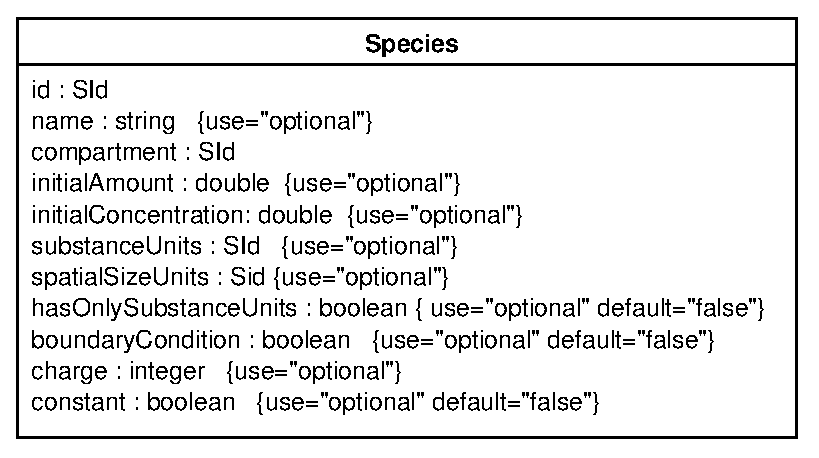
\includegraphics[scale=0.68]{species}
    &
    \begin{example}[c]
typedef struct
{
  char    *name;
  char    *compartment;
  double  initialAmount;
  char    *units;
  int     boundaryCondition;
  int     charge;
} Species_t;
    \end{example}\\
  \end{tabular}
  \caption{Definition of SBML Species in UML (left) and the
  corresponding \class{Species\_t} C struct (right).}
  \label{fig:species-uml-and-c}
\end{figure}

The mapping from SBML primitive types to C is straightforward as an
example will help illustrate.  A Species has at least one attribute of
every primitive type defined by SBML.
Figure~\ref{fig:species-uml-and-c} shows the UML definition for
Species and the corresponding C struct side-by-side.  The similarity
between the two demonstrates the mapping rules for primitive types:

\begin{enumerate}
  
  \item In all cases, the form of UML attribute names, including their
  capitalization, are preserved (e.g., \variable{initialAmount}) when
  mapped to C struct fields.

  \item SName maps to a standard C string (pointer to an array of
  characters terminated by a \texttt{NULL} (\texttt{0}) character; for
  e.g. \variable{char *name}).  Note that SName syntax is not yet
  enforced in the API.

  \item double and integer map to C \texttt{double} and \texttt{int}
  respectively.

  \item boolean maps to C \texttt{int}, where zero represents false
  and non-zero represents true.

\end{enumerate}


%-----------------------------------------------------------------------------
\subsection{Object Creation and Destruction}
%-----------------------------------------------------------------------------

This section and subsequent ones focus on functions or methods to
create, destroy and otherwise manipulate SBML C objects.  Since all
functions and methods follow the same naming convention, when
discussing them generically, \texttt{XXX} will be used to stand for
some class name and \texttt{YYY} some class attribute.


To instantiate (create) an object use either the
\method{XXX\_create()} or \method{XXX\_createWith()} constructor.  To
destroy (free) an object use \method{XXX\_free()}.  The constructors
and destructors for \class{Species} are:


\begin{methoddef}{Species\_t *Species\_create (void)}
  Creates a new Species and returns a pointer to it.
\end{methoddef}

\begin{methoddef}{Species\_t *Species\_createWith (const char *name,
const char *compartment,\\ double initialAmount, const char *units,
int boundaryCondition, int charge)}
  Creates a new Species with the given name, compartment,
  initialAmount, units, boundaryCondition and charge and returns a
  pointer to it.  This convenience function is functionally equivalent
  to:
  \begin{example}[c]
Species_t *s = Species_create();
Species_setName(s, name); Species_setCompartment(s, compartment); ...;
  \end{example}
\end{methoddef}

\begin{methoddef}{void Species\_free (Species\_t *s)}
  Frees the given Species.
\end{methoddef}


The \method{XXX\_createWith()} constructors are a convenient way both
to create SBML objects and initialize their attributes in a single
operation.  If \method{XXX\_create()} is used instead, only attributes
with default values (as defined by the specification) will be set.
All other attributes will default to zero in the case of integers and
doubles, false in the case of booleans or a NULL pointer in the case
of SNames strings.

When an SBML object is destroyed with \method{XXX\_free()}, all of its
Strings are freed (see Section~\ref{sec:accessing-fields}: Accessing
Fields for more information) and all of its contained objects are
freed (see Section~\ref{sec:lists}: Lists for more information).


%-----------------------------------------------------------------------------
\subsection{Accessing Fields}
\label{sec:accessing-fields}
%-----------------------------------------------------------------------------


%-----------------------------------------------------------------------------
\subsubsection{Getters}
%-----------------------------------------------------------------------------

There are two ways to get the value of a field within a struct: i)
direct reference and ii) via a method call.  Direct reference should
be preferred in almost all cases; it avoids the overhead of a function
call and thus is significantly faster\footnote{The getters are
\emph{not} \texttt{\#define} macros that are inlined at compilation
time.  They are true functions.}.  The getter methods are provided for
languages that do not allow direct access to the underlying C structs.
As an example of direct access, Figure~\ref{fig:print-species} lists a
function (which is not part of the API) to print the fields of a
\class{Species}.


\begin{figure}[htb]
  \begin{codeVerbatim}[C,flexiblecolumns=false]
/**
 * Prints Species to stream (good for debugging).
 */
void
myPrintSpecies (Species_t *s, FILE *stream)
{
  char none[]       = "(none)";
  char *compartment = (s->compartment == NULL) ? none : s->compartment;
  char *units       = (s->units       == NULL) ? none : s->units;
  char *boundary    = (s->boundaryCondition == 0) ? "false" : "true";


  fprintf(stream, "Species %s:\n", s->name);
  fprintf(stream, "         Compartment: %s\n", compartment      );
  fprintf(stream, "      Initial Amount: %f\n", s->initialAmount );
  fprintf(stream, "               Units: %s\n", units            );
  fprintf(stream, "  Boundary Condition: %s\n", boundary         );
  fprintf(stream, "              Charge: %d\n", s->charge        );
}
  \end{codeVerbatim}
  \caption{Demonstrates direct access to the fields of an SBML object,
  in this case \class{Species\_t}.}
  \label{fig:print-species}
\end{figure}

The getter methods follow the naming convention
\method{XXX\_getYYY()}.  The getters for Species are:


\begin{methoddef}{const char *Species\_getName (const Species\_t *s)}
  Returns the name of this Species.
\end{methoddef}

\begin{methoddef}{const char *Species\_getCompartment (const Species\_t *s)}
  Returns the compartment of this Species.
\end{methoddef}

\begin{methoddef}{double Species\_getInitialAmount (const Species\_t *s)}
  Returns the initialAmount of this Species.
\end{methoddef}

\begin{methoddef}{const char *Species\_getUnits (const Species\_t *s)}
  Returns the units of this Species.
\end{methoddef}

\begin{methoddef}{int Species\_getBoundaryCondition (const Species\_t *s)}
  Returns the boundaryCondition of this Species.
\end{methoddef}

\begin{methoddef}{int Species\_getCharge (const Species\_t *s)}
  Returns the charge of this Species.
\end{methoddef}

Notice the \class{Species\_t} passed to each getter is
\texttt{const}ant.  The purpose of this \texttt{const}ness is twofold:
i) it reinforces the notion that a getter simply returns a value and
does not modify the state of the passed-in object and ii) as a result,
in certain contexts a compiler may be able to use this information to
perform certain optimizations.  Notice also, whenever a getter returns
a string, it is constant (\texttt{const char *}), i.e. it cannot be
modified or freed.  The reason for this is each struct tracks and owns
all of its internal memory.  To modify (or especially free) this
memory without using one of the sanctioned access methods could be
particularly disasterous (most likely resulting in a segmentation or
general protection fault).  Memory management issues are elaborated
when discussing setters.


%-----------------------------------------------------------------------------
\subsubsection{Setters}
%-----------------------------------------------------------------------------

A value is assigned to a field via a set method\footnote{Earlier
versions of \textsc{libsbml} allowed primitive types to be set
directly.  Such direct access, however, made it impossible to
distinguish between set and unset states of a field, since all
possible values are valid (i.e. no sentinel value exists to indicate
an unset state).}.  Requiring all assignments to take place through a
setter allows \textsc{libsbml} to track (and the developer to query)
the set or unset \emph{state} of a field apart from its actual
\emph{value}.  The need to make a distinction between state and value
is critical and is discussed further in
Section~\ref{sec:field-states}.

The setter methods follow the naming convention
\method{XXX\_setYYY()}.  The setters for Species are:


\begin{methoddef}{void Species\_setName (Species\_t *s, const char *sname)}
  Sets the name of this Species to a copy of sname.
\end{methoddef}

\begin{methoddef}{void Species\_setCompartment (Species\_t *s,
const char *sname)}
  Sets the compartment of this Species to a copy of sname.
\end{methoddef}

\begin{methoddef}{void Species\_setInitialAmount (Species\_t *s, double value)}
  Sets the initialAmount of this Species to value and marks the
  field as set.
\end{methoddef}

\begin{methoddef}{void Species\_setUnits (Species\_t *s, const char *sname)}
  Sets the units of this Species to a copy of sname.
\end{methoddef}

\begin{methoddef}{void Species\_setBoundaryCondition (Species\_t *s, int value)}
  Sets the boundaryCondition of this Species to value (boolean) and marks
  the field as set.
\end{methoddef}

\begin{methoddef}{void Species\_setCharge (Species\_t *s, int value)}
  Sets the charge of this Species to value and marks the field as set.
\end{methoddef}


In the case of strings, requiring setter methods also enables clean
and simple memory semantics.  The rule is: every SBML object is
responsible for its own memory, including SName strings.  Whenever a
set method is called, the passed-in string is copied and stored.  If
the field being set previously contained a string, it is freed.  When
\method{XXX\_free()} is called, all strings are freed.

For example, to set the compartment of Species \variable{s} to the
string ``cell'':

\begin{example}[c]
Species_setCompartment(s, "cell");
\end{example}

The effect of passing a \texttt{NULL} pointer as the string argument
is to free the previously stored string and mark the field as unset.
The preferred method for doing this, however, is to use the
\method{XXX\_unsetYYY()} class of methods (see
Section~\ref{sec:field-states}).

There is nothing in C language specification or the compiler that
prevents string fields (or any other field type for that matter) from
being set directly, as in:

\begin{example}[c]
s->name = "s2";
\end{example}

But to do so would likely cause a memory leak if \texttt{s->name} was
already assigned to another string.  Using the setter methods is much
safer than assigning the memory directly and enables the set versus
unset state of the field to be tracked.


%-----------------------------------------------------------------------------
\subsubsection{Field States}
\label{sec:field-states}
%-----------------------------------------------------------------------------

For each optional field without a default value, \textsc{libsbml}
tracks both its state and value.  The state of a field indicates
whether the field is set (contains a valid value) or unset (contains
no value at all).  As mentioned before, the distinction between a set
and unset field is critical for both \textsc{libsbml} and applications
that depend upon it to function correctly (in accordance with the SBML
specifications).  Take for example the case of outputting SBML for a
\class{Species}.  \class{Species} has an optional charge attribute,
which means it need not ever be read-in (specified), written or
manipulated.  For this reason, \libsbml{} must be able to
determine the set or unset state of the \variable{charge} field to
either output or omit the field as appropriate.

The easiest way to determine whether a particular field in a structure is
set or unset is to use the \method{XXX\_isSetYYY()} class of methods.  For
Species, the following are available:


\begin{methoddef}{int Species\_isSetName (const Species\_t *s)}
  Return 1 if the name of this Species has been set, 0 otherwise.  In
  SBML L1, a Species name is required and therefore \textbf{should
  always be set}.  In L2, name is optional and as such may or may not
  be set.
\end{methoddef}

\begin{methoddef}{int Species\_isSetCompartment (const Species\_t *s)}
  Return 1 if the compartment of this Species has been set, 0 otherwise.
\end{methoddef}

\begin{methoddef}{int Species\_isSetInitialAmount (const Species\_t *s)}
  Returns 1 if the initialAmount of this Species has been set, 0
  otherwise.  In SBML L1, a Species initialAmount is required and
  therefore \textbf{should always be set}.  In L2, initialAmount is
  optional and as such may or may not be set.
\end{methoddef}

\begin{methoddef}{int Species\_isSetUnits (const Species\_t *s)}
  Returns 1 if the units of this Species has been set, 0 otherwise.
\end{methoddef}

\begin{methoddef}{int Species\_isSetCharge (const Species\_t *s)}
  Returns 1 if the charge of this Species has been set, 0 otherwise.
\end{methoddef}


Fields with default values do not have an \method{isSetYYY()}.  If the
value for such a field is never supplied by an SBML document or user,
the default is used. Therefore, if an \method{isSetYYY()} method did
exist, it would always return true (1).

Required fields, on the other hand, do have \method{isSetYYY()}
methods.  There are two points worth mentioning here.  First, it is
possible that a value for a required field is not given and a program
may want to check for and handle this case (especially if the program
is an SBML validator).  Second, please be aware from SBML Level 1 to
Level 2, some fields changed from required to optional.  If this is
the case for a particular field the method documentation will state it
(as above).  That said, this second point is more relevant when it
comes to unsetting fields.

Just as fields may be set and their set state queried, they may also
be unset.  Unset methods are named (predictably)
\method{XXX\_unsetYYY()}.  The unset methods for Species are:

\begin{methoddef}{void Species\_unsetName (Species\_t *s)}
  Unsets the name of this Species.  This is equivalent to the following code:\\
  \texttt{safe\_free(s->name); s->name = NULL;}
  \\
  In SBML L1, a Species name is required and therefore \textbf{should
  always be set}.  In L2, name is optional and as such may or may not
  be set.
\end{methoddef}

\begin{methoddef}{void Species\_unsetInitialAmount (Species\_t *s)}
  Unsets the initialAmount of this Species.  In SBML L1, a Species
  initialAmount is required and therefore \textbf{should always be
  set}.  In L2, initialAmount is optional and as such may or may not
  be set.
\end{methoddef}

\begin{methoddef}{void Species\_unsetUnits (Species\_t *s)}
  Unsets the units of this Species.  This is equivalent to:\\
  \texttt{safe\_free(s->units); s->units = NULL;}
\end{methoddef}

\begin{methoddef}{void Species\_unsetCharge (Species\_t *s)}
  Unsets the charge of this Species.
\end{methoddef}

Again, for the reason mentioned above, fields with default values do
not have \method{unsetYYY()} methods.  Similarly, required fields have
\method{unsetYYY()} methods only if they are declared optional in at
least one of SBML Level 1 and Level 2.  Notice, for example, there is
an \method{isSetCompartment()} method but no corresponding
\method{unsetCompartment()} (a compartment is required for a Species
in both SBML Level 1 and Level 2).

It is also possible to check the set status of a field directly.  For
SName strings this is simple, unset fields will contain a
\texttt{NULL} pointer:

\begin{example}[c]
  s->units != NULL  /* Equivalent to Species_isSetUnits(s). */
\end{example}

For primitive types things are only slightly more complicated.  A
nested \variable{isSet} struct of one bitfield per primitive type is
used to keep track of set states.  The value of a bitfield field is
one if corresponding field is set and zero otherwise.  The
\variable{isSet} struct was omitted from the definition of
\class{Species\_t} in Figure~\ref{fig:species-uml-and-c} to simplify
the explanation of getter methods.  A more complete definition of
\class{Species\_t}, with its \variable{isSet} nested struct is shown
in Figure~\ref{fig:species-isSet}.


So, to determine if a given species \variable{s} has a charge:

\begin{example}[c]
  s->isSet.charge == 1  /* Equivalent to Species_isSetCharge(s) */
\end{example}


\begin{figure}[bth]
  \begin{codeVerbatim}[C,flexiblecolumns=false]
typedef struct
{
  char    *name;
  char    *compartment;
  double  initialAmount;
  char    *units;
  int     boundaryCondition;
  int     charge;

  struct
  {
    unsigned int initialAmount:1;
    unsigned int charge       :1;
  } isSet;

} Species_t;
  \end{codeVerbatim}
  \caption{Definition of \class{Species\_t} C struct, including its
  nested \variable{isSet} struct of bitfields, used to track the state
  of primitive types.}
  \label{fig:species-isSet}
\end{figure}


%-----------------------------------------------------------------------------
\subsection{Lists}
\label{sec:lists}
%-----------------------------------------------------------------------------

\class{Species} contains only SNames and primitive types, but many
SBML classes also contain lists of other objects.  For example, a
\class{UnitDefinition} contains a list of \class{Units}:


\begin{figure}[h]
  \centering
  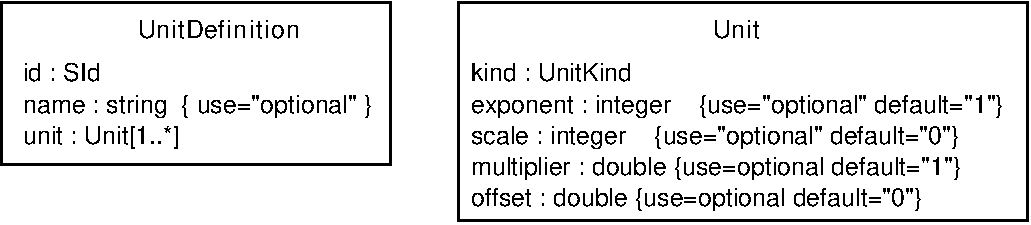
\includegraphics[scale=0.68]{unitdefinition}
  \label{fig:unit-definition}
\end{figure}


To help manage this containment relationship, three standard functions are
provided by \libsbml{}: \method{XXX\_addYYY()}, \method{XXX\_getYYY()} and
\method{XXX\_getNumYYY()}.  For example, the methods for UnitDefinition
are:


\begin{methoddef}{void UnitDefinition\_addUnit (UnitDefinition\_t *ud,
Unit\_t *u)}
  Adds the given Unit to this UnitDefinition.
\end{methoddef}

\begin{methoddef}{Unit\_t *UnitDefinition\_getUnit (const UnitDefinition\_t
*ud, unsigned int n)}
Returns the nth Unit of this UnitDefinition.
\end{methoddef}

\begin{methoddef}{unsigned int UnitDefinition\_getNumUnits (const
UnitDefinition\_t *ud)}
  Return the number of Units in this UnitDefinition.
\end{methoddef}


Furthering the example, creating the \class{UnitDefinition} $mmol l^-1
s^1$ named ``mmls'', corresponding to the SBML:

\begin{example}
<listOfUnitDefinitions>
  <unitDefinition name="mmls">
    <listOfUnits>
      <unit kind="mole"   scale="-3"/>
      <unit kind="litre"  exponent="-1"/>
      <unit kind="second" exponent="-1"/>
    </listOfUnits>
  </unitDefinition>
</listOfUnitDefinitions>
\end{example}


could be accomplished with the following C:

\begin{example}[c]
UnitDefinition_t *ud = UnitDefinition_createWith("mmls");

UnitDefinition_addUnit(ud, Unit_createWith(UNIT_KIND_MOLE  ,  1, -3) );
UnitDefinition_addUnit(ud, Unit_createWith(UNIT_KIND_LITRE , -1,  0) );
UnitDefinition_addUnit(ud, Unit_createWith(UNIT_KIND_SECOND, -1,  0) );
\end{example}


In this case, \method{UnitDefinition\_getNumUnits(\variable{ud})}
returns 3 and \method{UnitDefinition\_getUnit(\variable{ud}, 1)}
returns the \emph{second} Unit\footnote{(The UNIT\_KIND\_XXX
enumerations are discussed later.}.  Notice that items are numbered
starting at zero.

Related to lists is a set of convenience methods for creating and
adding SBML objects to a \class{Model} in a single operation.  The
rationale is that since a \class{Model} is the top-level container for
all other SBML objects, programmers are likely to have handles to
them.  Another way to construct the above \class{UnitDefinition}, but
this time inside a \class{Model}, is:


\begin{example}[c]
Model_t            *m  = Model_createWith("MyModel");
UnitDefinition_t   *ud = Model_createUnitDefinition(m);

UnitDefinition_setName(ud, "mmls");

Model_createUnit(m, Unit_createWith(UNIT_KIND_MOLE  ,  1, -3) );
Model_createUnit(m, Unit_createWith(UNIT_KIND_LITRE , -1,  0) );
Model_createUnit(m, Unit_createWith(UNIT_KIND_SECOND, -1,  0) );
\end{example}


\method{Model\_createUnit()} creates a new Unit inside the Model
\variable{m} and returns a pointer to it (in this case the result is
discarded).  The \class{Unit} is added to the last
\class{UnitDefinition} created.  One caveat to be aware of with these
methods is the case where no intermediate container exists; e.g., if
no \class{UnitDefinition} were created above.  In that case, the call
to \method{Model\_createUnit()} does nothing.  More specifically, no
\class{Unit} is created and (obviously) nothing is added to the model.

For more detailed information on Lists, see Appendix~\ref{app:lists}.


%-----------------------------------------------------------------------------
\subsection{Enumerations}
\label{sec:enumerations}
%-----------------------------------------------------------------------------

SBML has two enumeration types, \texttt{UnitKind} and
\texttt{RuleType}.  These translate directly to C \texttt{enum}s with a
few support functions for equality testing and converting to and from
strings.  From \texttt{UnitKind.h}:


\begin{example}[c]
typedef enum
{
    UNIT_KIND_AMPERE
  , UNIT_KIND_BECQUEREL
  , UNIT_KIND_CANDELA

   /* Omitted for space */

  , UNIT_KIND_WATT
  , UNIT_KIND_WEBER
  , UNIT_KIND_INVALID
} UnitKind_t;
\end{example}


\begin{methoddef}{int UnitKind\_equals (UnitKind\_t uk1, UnitKind\_t uk2)}
  Tests for logical equality between two UnitKinds.  This function behaves
  exactly like C's \texttt{==} operator, except for the following two cases:

\begin{itemize}
  \item \texttt{UNIT\_KIND\_LITER == UNIT\_KIND\_LITRE}
  \item \texttt{UNIT\_KIND\_METER == UNIT\_KIND\_METRE}
\end{itemize}

  where C would yield false (since each of the above is a distinct
  enumeration value), \method{UnitKind\_equals(...)} yields true.
  Returns true (!0) if uk1 is logically equivalent to uk2, false (0)
  otherwise.
\end{methoddef}
  
\begin{methoddef}{UnitKind\_t UnitKind\_forName (const char *name)}
  Returns the UnitKind with the given name (case-insensitive).
\end{methoddef}

\begin{methoddef}{const char *UnitKind\_toString (UnitKind\_t uk)}
  Returns the name of the given UnitKind.  The caller does not own the
  returned string and is therefore not allowed to modify it.
\end{methoddef}

The last item in the enumeration, \class{UNIT\_KIND\_INVALID}, is used
whenever, as the name implies, the \class{UnitKind} is invalid or
unknown.  The corresponding string representation is ``(Invalid
UnitKind)''.  When a Unit is created, its kind field is initialized to
\class{UNIT\_KIND\_INVALID}.  Also, \method{UnitKind\_forName()} will
return \class{UNIT\_KIND\_INVALID} if the passed-in name does not
match any known \class{UnitKind}.

The same ideas apply to \class{ RuleType}, except there is no need for
\method{RuleType\_equals()}.  See \texttt{RuleType.h} for more
information.

\subsubsection{Note:}

The internal \variable{UNIT\_KIND\_STRINGS} table is sorted
alphabetically and \class{UnitKind\_t} matches this sort order.
Because of this, \method{UnitKind\_forName()} is able to perform a
binary search to find a matching name, making its complexity
$O(log(n))$.  That is, \method{UnitKind\_forName()} is implemented
efficiently.


%-----------------------------------------------------------------------------
\subsection{Abstract Classes}
\label{sec:abstract-classes}
%-----------------------------------------------------------------------------

The SBML specification defines three classes that have no
representation apart from subclasses that specialize (inherit from)
them.  In OOP parlance, these types are termed abstract.  The abstract
SBML classes are:


\begin{table}[bth]
  \centering
  \begin{tabular}{ll}
    \toprule
    \textbf{SBML Class}         & \textbf{C Class (typedef struct)} \\
    \midrule
    \emph{SBase}                & \class{SBase\_t}                  \\
    \emph{Rule}                 & \class{Rule\_t}                   \\
    \emph{AssignmentRule}       & \class{AssignmentRule\_t}         \\
    \bottomrule
  \end{tabular}
  \caption{Abstract SBML classes their corresponding C class.}
  \label{tab:sbml-abstract-classes}
\end{table}


The conventions for abstract classes in the \textsc{libsbml} API are
similar to that of other classes with a few modifications and
additions.

Since abstract classes cannot be created or destroyed directly, they
have no \method{XXX\_create()} or {XXX\_free()} methods.  Instead they
have \method{XXX\_init()} and \method{XXX\_clear()} methods which
subclasses use to initialize and free their memory, respectively.
Users of the API do not need to worry about these functions.

Fields of the abstract class are \texttt{\#define}d to a symbol in the
class header file.  This symbol is used in subclasses \emph{in the order of
inheritance}.  For example, Species inherits from SBase:


\begin{figure}[h]
  \centering
  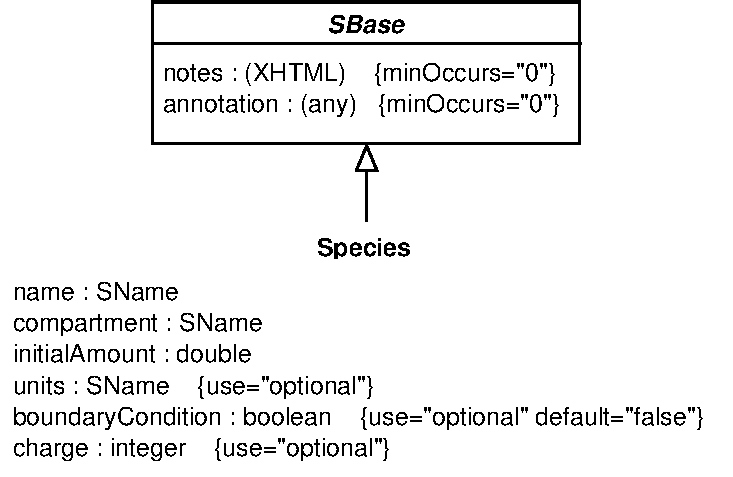
\includegraphics[scale=0.68]{sbase-species}
  \label{fig:sbase-species}
\end{figure}


\texttt{SBase.h} defines:


\begin{example}[c]
/**
 * As shown below, put SBASE_FIELDS as the *first* item of any struct
 * which "is a(n)" SBML object.
 */
#define SBASE_FIELDS          \
  SBMLTypeCode_t typecode; \
  char             *notes;    \
  char             *annotation
\end{example}


and recall \class{Species\_t} from earlier:

\begin{example}[c]
typedef struct
{
  SBASE_FIELDS;
  char   *name;
  char   *compartment;
  double  initialAmount;
  char   *units;
  int     boundaryCondition;
  int     charge;
} Species_t;
\end{example}

The effect is that when the library source is compiled, the first
three fields of \class{Species} are \variable{typecode},
\variable{notes}, and \variable{annotation}.  In fact, every class
that inherits from \class{SBase}, i.e. all SBML classes, have these
same first three fields.  Accessing the notes or annotation field of a
\class{Species\_t} \variable{*s}, or any other SBML object, is the
same as for other fields.  For example:

\begin{example}[c]
if (s->notes != NULL)
{
  printf("Notes for Species %s:\n", (s->name == NULL) ? "(null)" : s->name);
  printf("%s", s->notes);
}
\end{example}

Setting string fields requires special care to guard against memory
leaks.  The \method{XXX\_setYYY()} methods must be used.  But,
\class{Species} does not define either the notes or annotation fields
and as such there are \emph{no} \method{Species\_setNotes()} or
\method{Species\_setAnnotation()} methods.  Instead, \class{SBase}
defines them:

\begin{methoddef}{void SBase\_setNotes (SBase\_t *sb, const char *notes)}
  Sets the notes field of the given SBML object to a copy of notes.
  If object already has notes, the existing string is freed before the
  new one is copied.
\end{methoddef}

\begin{methoddef}{void SBase\_setAnnotation (SBase\_t *sb, const char
*annotation)}
  Sets the annotation field of the given SBML object to a copy of
  annotations.  If object already has an annotation, the existing string
  is freed before the new one is copied.
\end{methoddef}


The first argument to these functions is, of course, an object of type
\class{SBase}.  Since \class{Species} inherits from \class{SBase},
i.e. \class{Species} \emph{is an} \class{SBase}, it can be used as the
first argument to these functions.  A slight caveat is a cast is
required.  To set the notes field of \class{Species} \variable{s}
then:


\begin{example}[c]
SBase_setNotes( (SBase_t *) s, "My Favorite Species" );
\end{example}


The same applies to all other SBML objects.


Finally, each SBML class has a \variable{typecode} which is
initialized when an object is instantiated.  The \variable{typecode}
is a simple C enumeration, defined in \texttt{SBMLTypeCodes.h}:


\begin{example}[c]
/**
 * An enumeration of SBML types to help identify SBML objects at runtime.
 * Abstract types do not have a typecode since they cannot be instantiated.
 */
typedef enum
{
    SBML_COMPARTMENT
  , SBML_KINETIC_LAW
  , SBML_MODEL
  , SBML_PARAMETER
  , SBML_REACTION
  , SBML_SPECIES
  , SBML_SPECIES_REFERENCE
  , SBML_UNIT_DEFINITION
  , SBML_UNIT
  , SBML_ALGEBRAIC_RULE
  , SBML_SPECIES_CONCENTRATION_RULE
  , SBML_COMPARTMENT_VOLUME_RULE
  , SBML_PARAMETER_RULE
} SBMLTypeCode_t;
\end{example}

The primary reason for the \variable{typecode} is distinguish specific
types of rules in a Model.  A \class{Model} contains a list of rules,
but a \class{Rule} in SBML may be of one of four specific types:
\class{AlgebraicRule}, \class{SpeciesConcentrationRule},
\class{CompartmentVolumeRule} and \class{ParameterRule}.




%=============================================================================
\section{Reading SBML Files}
\label{sec:reading-sbml}
%=============================================================================

SBML may be read from a file or an in memory string into an
SBMLDocument.  \texttt{SBMLReader.h} defines two basic read functions:

\begin{methoddef}{SBMLDocument\_t *readSBML (const char *filename)}
  Reads the SBML document from the given file and returns a pointer to
  it.
\end{methoddef}

\begin{methoddef}{SBMLDocument\_t *readSBMLFromString (const char *xml)}
  Reads the SBML document from the given XML string and returns a pointer
  to it.

  The XML string must be complete and legal XML document.  Among other
  things, it must start with an XML processing instruction.  For e.g.,:
  \begin{example}
    <?xml version='1.0' encoding='UTF-8'?>
  \end{example}
\end{methoddef}


These functions return a pointer to an SBMLDocument:


\begin{example}[c]
/**
 * The SBMLDocument
 */
typedef struct
{
  unsigned int level;
  unsigned int version;

  List_t *error;
  List_t *fatal;
  List_t *warning;

  Model_t *model;
} SBMLDocument_t;
\end{example}


The level and version of the SBML document are stored in the first two
fields.  The last field is the SBML model itself.  The three lists
record warnings and errors encountered during the XML parse.  Each
warning or error is a ParseMessage (again from
\texttt{SBMLDocument.h}):


\begin{example}[c]
/**
 * SBMLDocuments contain three Lists of ParseMessages, one for each class
 * of messages that could be triggered during an XML parse: Warnings,
 * Errors and Fatal Errors.
 *
 * Each ParseMessage contains the message itself and the line and column
 * numbers of the XML entity that triggered the message.  If line or column
 * information is unavailable, -1 is used.
 */
typedef struct
{
  char *message;
  int  line;
  int  column;
} ParseMessage_t;
\end{example}


While its possible to access these lists directly, convenience
functions are provided:


\begin{methoddef}{ParseMessage\_t *SBMLDocument\_getWarning
(SBMLDocument\_t *d, unsigned int n)}
   Returns the nth warning encountered during the parse of this
   SBMLDocument or \texttt{NULL} if \texttt{n > getNumWarnings() - 1}.
 \end{methoddef}

\begin{methoddef}{ParseMessage\_t *SBMLDocument\_getError (SBMLDocument\_t *d,
unsigned int n);}
   Returns the nth error encountered during the parse of this
   SBMLDocument or \texttt{NULL} if \texttt{n > getNumErrors() - 1}.
 \end{methoddef}

\begin{methoddef}{ParseMessage\_t *SBMLDocument\_getFatal (SBMLDocument\_t *d,
unsigned int n)}
   Returns the nth fatal error encountered during the parse of this
   SBMLDocument or \texttt{NULL} if \texttt{n > getNumErrors() - 1}.
 \end{methoddef}


\begin{methoddef}{unsigned int SBMLDocument\_getNumWarnings
(SBMLDocument\_t *d)}
   Returns the number of warnings encountered during the parse of this
   SBMLDocument.
 \end{methoddef}

\begin{methoddef}{unsigned int SBMLDocument\_getNumErrors (SBMLDocument\_t *d)}
   Returns the number of errors encountered during the parse of this
   SBMLDocument.
 \end{methoddef}

\begin{methoddef}{unsigned int SBMLDocument\_getNumFatals (SBMLDocument\_t *d)}
   Returns the number of fatal errors encountered during the parse of this
   SBMLDocument.
 \end{methoddef}
  

\begin{methoddef}{void SBMLDocument\_printWarnings (SBMLDocument\_t *d,
FILE *stream)}
  Prints all warnings encountered during the parse of this SBMLDocument to
  the given stream.  If no warnings have occurred, i.e.
  \texttt{SBMLDocument\_getNumWarnings(d) == 0}, no output will be sent to
  stream. The format of the output is:
  \begin{example}
    %d Warning(s):
      Line %d, Col %d: %s
      ...
  \end{example}
  This is a convenience function to aid in debugging.  For example:\\
  \texttt{SBMLDocument\_printWarnings(d, stdout)}.
 \end{methoddef}
  

\begin{methoddef}{void SBMLDocument\_printErrors (SBMLDocument\_t *d,
FILE *stream)}
  Prints all errors encountered during the parse of this SBMLDocument
  to the given stream.  If no errors have occurred, that is, if 
  \texttt{SBMLDocument\_getNumErrors(d) == 0}, no output will be sent
  to stream. The format of the output is:
  \begin{example}
    %d Error(s):
      Line %d, Col %d: %s
      ...
  \end{example}
  This is a convenience function to aid in debugging.  For example:\\
  \texttt{SBMLDocument\_printErrors(d, stdout)}.
 \end{methoddef}
  

\begin{methoddef}{void SBMLDocument\_printFatals (SBMLDocument\_t *d,
FILE *stream)}
  Prints all fatals encountered during the parse of this SBMLDocument
  to the given stream.  If no fatals have occurred, that is, if
  \texttt{SBMLDocument\_getNumFatals(d) == 0}, no output will be sent
  to stream. The format of the output is:
  \begin{example}
    %d Fatal(s):
      Line %d, Col %d: %s
      ...
  \end{example}
  This is a convenience function to aid in debugging.  For example:\\
  \texttt{SBMLDocument\_printFatals(d, stdout)}.
 \end{methoddef}


%-----------------------------------------------------------------------------
\subsection{A Simple Example}
\label{sec:read-example}
%-----------------------------------------------------------------------------

The following example is included in the distribution as
\texttt{readSBML.c}.  It is compiled as part of the build process, but
is not installed.  The program takes a single command-line argument,
the name of an SBML file, reads it into memory and reports some basic
information about the file: warnings or errors (if any are reported)
as well as the total read time (in milliseconds).

To run the example, go to the top-level directory where
\textsc{libsbml} was unpacked and:

\begin{example}[csh]
  % cd src
  % ./readSBML test-data/l1v1-branch.xml
  % ./readSBML test-data/l1v1-minimal.xml
  % ./readSBML test-data/l1v1-rules.xml
  % ./readSBML test-data/l1v1-units.xml
  % # etc...
\end{example}


The exact procedure for compile the example (and linking-in
\textsc{libsbml} in general) varies from one platform and compiler to
another.  On Linux or Solaris with GCC the following should work:

\begin{example}[csh]
  % gcc -o readSBML readSBML.c -lsbml
\end{example}


The example is listed below:

%\begin{figure}[hbt]
\begin{codeVerbatim}[C,flexiblecolumns=false]
#include <stdio.h>
#include <sys/time.h>

#include "sbml/SBMLReader.h"
#include "sbml/SBMLTypes.h"

/**
 * Function Prototypes
 */
unsigned long getCurrentMillis (void);
void          reportErrors     (SBMLDocument_t *d);


int
main (int argc, char *argv[])
{
  SBMLDocument_t *d;
  Model_t *m;

  unsigned long start, stop;


  if (argc != 2)
  {
    printf("usage: readSBML <filename>\n");
    return 1;
  }

  start = getCurrentMillis();
  d     = readSBML(argv[1]);
  stop  = getCurrentMillis();

  m = d->model;

  printf( "File: %s\n", argv[1]);
  printf( "       model name: %s\n",  m->name );
  printf( "  unitDefinitions: %d\n",  Model_getNumUnitDefinitions(m) );
  printf( "     compartments: %d\n",  Model_getNumCompartments(m)    );
  printf( "          species: %d\n",  Model_getNumSpecies(m)         );
  printf( "       parameters: %d\n",  Model_getNumParameters(m)      );
  printf( "        reactions: %d\n",  Model_getNumReactions(m)       );
  printf( "            rules: %d\n",  Model_getNumRules(m)           );
  printf( "\n");

  printf( "Total Read Time (ms): %lu\n", stop - start);

  SBMLDocument_printWarnings(d, stdout);
  SBMLDocument_printErrors  (d, stdout);
  SBMLDocument_printFatals  (d, stdout);

  SBMLDocument_free(d);
  return 0;
}


/**
 * @return the number of milliseconds elapsed since the Epoch.
 */
unsigned long
getCurrentMillis (void)
{
  struct timeval tv;
  unsigned long  result = 0;


  if (gettimeofday(&tv, NULL) == 0)
  {
    result = (tv.tv_sec * 1000) + (tv.tv_usec * .001);
  }

  return result;
}
\end{codeVerbatim}

%\caption{Using \textsc{libsbml} to read an SBML file into memory and
%(minimally) inspect it.  The support function
%\texttt{getCurrentMillis()} is listed in
%Figure~\ref{fig:getCurrentMillis}.}
%\label{fig:readSBML-example}
%\end{figure}


%\begin{figure}[hbt]
%\begin{codeVerbatim}[C,flexiblecolumns=false]
%
%\end{codeVerbatim}
%\caption{This function is called by \texttt{readSBML.c} (see
%Figure~\ref{fig:readSBML-example}).}
%\label{fig:getCurrentMillis}
%\end{figure}


%-----------------------------------------------------------------------------
\subsection{XML Schema Validation}
\label{sec:schema-validation}
%-----------------------------------------------------------------------------

To validate an SBML document against an SBML (XML) schema as it is
being read-in requires creating an \texttt{SBMLReader} object and
setting the appropriate schema filename and validation level.  The
functions for doing this are:


\begin{methoddef}{SBMLReader\_t *SBMLReader\_create (void)}
  Creates a new SBMLReader and returns a pointer to it.  By default
  schema validation is off (\texttt{XML\_SCHEMA\_VALIDATION\_NONE})
  and \texttt{schemaFilename} is \texttt{NULL}.
\end{methoddef}

\begin{methoddef}{void SBMLReader\_free (SBMLReader\_t *sr)}
  Frees the given SBMLReader.
\end{methoddef}

\begin{methoddef}{void SBMLReader\_setSchemaFilename (SBMLReader\_t *sr,
const char *filename)} Sets the schema filename used by this
  SBMLReader.  The filename should be either i) an absolute path or
  ii) relative to the directory contain the SBML file(s) to be read.
\end{methoddef}


\begin{methoddef}{void SBMLReader\_setSchemaValidationLevel ( SBMLReader\_t *sr,
XMLSchemaValidation\_t level )}
  Sets the schema validation level used by this SBMLReader.

  The levels are:
  \begin{itemize}
    \item \texttt{XML\_SCHEMA\_VALIDATION\_NONE} (0) turns schema
    validation off.

    \item \texttt{XML\_SCHEMA\_VALIDATION\_BASIC} (1) validates an XML
    instance document against an XML Schema.  Those who wish to
    perform schema checking on SBML documents should use this option.

    \item \texttt{XML\_SCHEMA\_VALIDATION\_FULL} (2) validates both
    the instance document itself \emph{and} the XML Schema document.
    The XML Schema document is checked for violation of particle
    unique attribution constraints and particle derivation
    restrictions, which is both time-consuming and memory intensive.
  \end{itemize}
\end{methoddef}


Once an \texttt{SBMLReader} has been created, there two variants of the
functions \texttt{readSBML()} and \texttt{readSBMLFromString()} become
available.  These variants can be thought of as methods of the
\texttt{SBMLReader} class.


\begin{methoddef}{SBMLDocument\_t *SBMLReader\_readSBML (SBMLReader\_t *sr,
const char *filename)}
  Reads the SBML document from the given file and returns a pointer to
  it.
\end{methoddef}

\begin{methoddef}{SBMLDocument\_t *SBMLReader\_readSBMLFromString (SBMLReader\_t *sr, const char *xml)}
  Reads the SBML document from the given XML string and returns a pointer
  to it.

  The XML string must be complete and legal XML document.  Among other
  things, it must start with an XML processing instruction.  For e.g.,:
  \begin{example}
    <?xml version='1.0' encoding='UTF-8'?>
  \end{example}
\end{methoddef}


Schema violations are reported in the \texttt{SBMLDocument}'s list of
\texttt{ParseMessages}.


%=============================================================================
\section{Writing SBML Files}
\label{sec:writing-sbml}
%=============================================================================

The \texttt{SBMLWriter} class is similiar to the \texttt{SBMLReader}
class.  The difference with an \texttt{SBMLWriter} is instead of
selecting a schema filename and validation level, an output encoding
is chosen instead.  The supported output encodings are:


\begin{example}[c]
/**
 * The character encodings supported by SBMLWriter
 */
typedef enum
{
    CHARACTER_ENCODING_ASCII
  , CHARACTER_ENCODING_UTF_8
  , CHARACTER_ENCODING_UTF_16
  , CHARACTER_ENCODING_ISO_8859_1
  , CHARACTER_ENCODING_INVALID
} CharacterEncoding_t;
\end{example}


\texttt{SBMLWriter.h} defines the following functions:


\begin{methoddef}{SBMLWriter\_t *SBMLWriter\_create (void)}
  Creates a new SBMLWriter and returns a pointer to it. By default the
  character encoding is ISO 8859-1
  (\texttt{CHARACTER\_ENCODING\_ISO\_8859\_1}).
\end{methoddef}


\begin{methoddef}{void SBMLWriter\_free (SBMLWriter\_t *sw)}
  Frees the given SBMLWriter.
\end{methoddef}

\begin{methoddef}{void SBMLWriter\_setEncoding (SBMLWriter\_t *sw,
CharacterEncoding\_t encoding)}
  Sets the character encoding for this SBMLWriter to the given
  CharacterEncoding type.
\end{methoddef}

\begin{methoddef}{int SBMLWriter\_writeSBML (SBMLWriter\_t *sw,
SBMLDocument\_t *d, const char *filename )}
  Writes the given SBML document to filename (with the settings
  provided by this SBMLWriter).

  Returns 1 on success and 0 on failure (e.g., if filename could not
  be opened for writing or the SBMLWriter character encoding is
  invalid).
\end{methoddef}

\begin{methoddef}{char *SBMLWriter\_writeSBMLToString (SBMLWriter\_t *sw,
SBMLDocument\_t *d)}
  Writes the given SBML document to an in-memory string (with the
  settings provided by this SBMLWriter) and returns a pointer to it.
  The string is owned by the caller and should be freed (with
  \texttt{free()}) when no longer needed.

  Returns \texttt{NULL} on failure (e.g., if the SBMLWriter character
  encoding is invalid).
\end{methoddef}


Finally, if the default character encoding of ISO 8859-1 is acceptable,
there are two simpler equivalents to the above functions:


\begin{methoddef}{int writeSBML (SBMLDocument\_t *d, const char *filename)}
  Writes the given SBML document to filename with the settings provided by
  this SBMLWriter.  This convenience function is functionally equivalent
  to:

  \begin{example}[c]
    SBMLWriter_writeSBML(SBMLWriter_create(), d, filename);
  \end{example}

  Returns 1 on success and 0 on failure (e.g., if filename could not be
  opened for writing or the SBMLWriter character encoding is invalid).
\end{methoddef}


\begin{methoddef}{char *writeSBMLToString (SBMLDocument\_t *d)}
  Writes the given SBML document to an in-memory string (with the settings
  provided by this SBMLWriter) and returns a pointer to it.  The string is
  owned by the caller and should be freed (with free()) when no longer
  needed.  This convenience function is functionally equivalent to:
  
  \begin{example}[c]
    SBMLWriter_writeSBMLToString(SBMLWriter_create(), d);
  \end{example}

  Returns \texttt{NULL} on failure (e.g., if the SBMLWriter character
  encoding is invalid).
\end{methoddef}


%=============================================================================
\section{Handling of Mathematical Formulas and MathML}
\label{sec:mathml}
%=============================================================================

\libsbml{} can read and write MathML 2.0~\citep{w3c:2000b} content in SBML
documents and data streams, as well as translate between MathML and the
text-string formulas used in SBML Level~1.  This section describes the
MathML and mathematics handling capabilities of the library.


%-----------------------------------------------------------------------------
\subsection{Reading and Writing Formulas in Text-String Form}
\label{sec:text-string-math}
%-----------------------------------------------------------------------------

In SBML Level~1, mathematical formulas are expressed as text strings using
a simple C-like syntax.  In SBML Level~2, mathematical formulas are
expressed in MathML syntax.  The API interfaces to SBML files and data
streams work with ASCII text strings in both cases; the difference between
Level~1 and Level~2 mathematical expressions is entirely in the syntax of
the strings.

Whether formulas in SBML are expressed in the C-like syntax of Level~1 or
in the MathML syntax of Level~2, they are converted internally in
\libsbml{} into Abstract Syntax Trees (ASTs).  The structure of ASTs is
described in detail in Appendix~\ref{app:ast}.  When \libsbml{} reads an
SBML model, it converts the expressions into ASTs and stores the ASTs in
the corresponding data structures that have mathematical formulas (such as
in a \texttt{KineticLaw}).  Thus, the \method{KineticLaw\_getMath()} method,
for example, returns a pointer to the root of an AST corresponding to the
formula stored there.

Many software packages provide users with the ability to express formulas
for such things as reaction rate expressions, and these packages'
interfaces often let users type in the formulas directly as strings.
\libsbml{} provides two high-level functions for working with mathematical
expressions in the form of strings: \method{SBML\_parseFormula} and
\method{SBML\_formulaToString}.

\begin{methoddef}{ASTNode\_t *SBML\_parseFormula (const char *formula)}
  Parses the given string as a mathematical formula in SBML Level~1 syntax
  form, and returns a representation of it as an Abstract Syntax Tree
  (AST).  This function returns the root node of the AST.  If the formula
  contains a syntax error, this function returns NULL instead.
\end{methoddef}

\begin{methoddef}{char *SBML\_formulaToString (ASTNode\_t *tree)}
  Returns a text-string mathematical expression corresponding to the
  Abstract Syntax Tree given as the argument.  The caller owns the memory
  allocated for the returned string and is responsible for freeing it when
  it is no longer needed.
\end{methoddef}

Using these methods is exceedingly simple.  The following is a code
fragment that illustrates calling the parser function repeatedly with
different formula strings, taking the ASTs returned each time and handing
them back to the formula generator and comparing the strings to make sure
they matched.  (This is not something a real application would ever need to
do, but it does simply illustrate the use of these two methods.)

\begin{example}[c]
const char *formulae[] =
{
  "1",
  "2.1",
  "2.1e+10",
  "foo",
  "1 + foo",
  "1 + 2",
  "1 + 2 * 3",
  "(1 - 2) * 3",
  "1 + -2 / 3",
  "1 + -2e-100 / 3",
  "1 - -foo / 3",
  "2 * foo^bar + 3.1",
  "foo()",
  "foo(1)",
  "foo(1, bar)",
  "foo(1, bar, 2^-3)",
  ""
};

ASTNode_t *n;
char      *s;
int        i;

for (i = 0; i < *formulae[i]; i++)
{
  n = SBML_parseFormula( formulae[i] );  /* Convert string to AST */
  s = SBML_formulaToString(n);              /* Convert AST back to string */

  fail_unless( !strcmp(s, formulae[i]), NULL );

  ASTNode_free(n);
  safe_free(s);
}
\end{example}



%-----------------------------------------------------------------------------
\subsection{Reading Formulas in MathML Form}
\label{sec:mathml-math}
%-----------------------------------------------------------------------------

There may arise situations in which an application needs to convert MathML
directly into an AST.  \libsbml{} provides the utility function
\method{readMathMLFromString()} for this purpose.  

\begin{methoddef}{MathMLDocument\_t *readMathMLFromString (const char *xml)}
  Reads a string containing an XML MathML expression, constructs the
  corresponding Abstract Syntax Tree and returns a pointer to a
  \class{MathMLDocument\_t} holding the tree structure.
\end{methoddef}

The object returned by \method{readMathMLFromString()} is a simple
container for an AST.  The class of this object, MathMLDocument, is not
defined by the SBML language standard but is provided in \libsbml{} as a
utility class.  MathMLDocument serves as a top-level container for XML
documents containing only MathML; in some ways it mirrors the SBMLDocument
class, which acts as a container for XML documents containing SBML.  The
definition of \class{MathMLDocument\_t} is as follows:
 
\begin{example}[c]
/**
 * The MathMLDocument
 */
typedef struct
{
  ASTNode_t *math;
} MathMLDocument_t;
\end{example}  

The following are the functions defined for the MathMLDocument class:

\begin{methoddef}{MathMLDocument\_t *MathMLDocument\_create ()}
  Creates a \class{MathMLDocument\_t} object structure.
\end{methoddef}

\begin{methoddef}{void MathMLDocument\_free (MathMLDocument\_t *d)}
  Frees the given \class{MathMLDocument\_t} structure.
\end{methoddef}

\begin{methoddef}{ASTNode\_t *MathMLDocument\_getMath (const MathMLDocument\_t *d)}
  Returns the Abstract Syntax Tree representation of the mathematical
  formula stored in this \class{MathMLDocument\_t} structure.
\end{methoddef}

Note that because the content passed to \method{readMathMLFromString()} is
handed to an XML parser, the string given as argument must be a complete
XML document.  The following example illustrates the use of this function
with a valid MathML input.

\begin{example}[c]
MathMLDocument_t *D;

const char* s = "<?xml version='1.0' encoding='ascii'?>"
                  "<math xmlns='http://www.w3.org/1998/Math/MathML'>"
                  "<apply><arccos/><ci> x </ci></apply>"
                  "</math>";

D = readMathMLFromString(s);
\end{example}


%-----------------------------------------------------------------------------
\subsection{Special Cases in Mathematical Formulas}
\label{sec:mathml-special-cases}
%-----------------------------------------------------------------------------





\clearpage
\appendix
%=============================================================================
\section{Lists}
\label{app:lists}
%=============================================================================

While List convenience methods (e.g., \texttt{XXX\_getNumYYY()}) are
provided for every class, it is possible to access and manipulate each
list directly.  All lists are themselves objects of type
\texttt{List\_t}.  The full set of list methods are:


\begin{methoddef}{void List\_add (List\_t *list, void *item)}
  Adds item to this List.
\end{methoddef}

\begin{methoddef}{void *List\_get (List\_t *list, unsigned int n)}
  Returns the nth item in this List.  If \texttt{n > List\_size(list)
  - 1} returns \texttt{NULL}.
\end{methoddef}

\begin{methoddef}{void *List\_remove (List\_t *list, unsigned int n)}
  Removes the nth item from this List and returns a pointer to it.  If
  \texttt{n > List\_size(list) - 1} returns \texttt{NULL}.
\end{methoddef}

\begin{methoddef}{unsigned int List\_size (List\_t *list)}
  Returns the number of elements in this List.
\end{methoddef}


Since UnitDefinitions maintains a List of Units, the UnitDefinition
example in Section~\ref{sec:lists} could also be written as:


\begin{example}[c]
UnitDefinition_t *ud = UnitDefinition_createWith("mmls");

List_add(ud->unit, Unit_createWith(UNIT_KIND_MOLE  ,  1, -3) );
List_add(ud->unit, Unit_createWith(UNIT_KIND_LITRE , -1,  0) );
List_add(ud->unit, Unit_createWith(UNIT_KIND_SECOND, -1,  0) );
\end{example}


However, this approach is not preferred.  The best reason to use
specific \texttt{XXX\_getYYY()} methods over the List API is that the
former are typed to specific items, whereas \texttt{List\_get()}
returns a void pointer that must be cast to a specific type.  For
example, compare:

\begin{example}[c]
Unit_t *u = UnitDefinition_getUnit(u, 1);
\end{example}

to:

\begin{example}[c]
Unit_t *u = (Unit_t *) List_get(ud->unit, 1);
\end{example}

Further, the first is more readable.  The List API is mentioned i) for
the sake of completeness and ii) currently the only way to remove an
item from a list is to use the API directly:

\begin{example}[c]
List_remove(ud->unit, 2);
\end{example}

has no analog in UnitDefinition.  ``Remove'' convenience methods can be
added to the API.  This feature was skipped because list item removal
seemed like an uncommon operation.


%=============================================================================
\section{Abstract Syntax Trees and \texttt{ASTNode\_t}}
\label{app:ast}
%=============================================================================

Abstract Syntax Trees (ASTs) in \libsbml{} are a simple data structure for
storing mathematical expressions.  For many applications, the details of
ASTs are irrelevant because the applications can use the text-string based
translation functions described in Sections~\ref{sec:text-string-math} and
\ref{sec:mathml-math}.  However, other applications do need to read and
manipulate ASTs directly.  This section describes \libsbml{}'s AST in
sufficient detail so software authors can write code to work with them.

An AST \emph{node} is a recursive structure containing a pointer to the
node's value (e.g., a number or a symbol) and a list of children nodes.
The following is the definition of \class{ASTNode\_t}:

\begin{example}[c]
/**
 * An Abstract Syntax Tree (AST) node.
 */
typedef struct
{
  ASTNodeType_t type;

  union
  {
    char   ch;
    char   *name;
    long   integer;
    double real;
  } value;    

  union
  {
    long denominator;
    long exponent;
  } extra;

  List_t *children;
} ASTNode_t;
\end{example}

For nodes containing character, string, integer, or simple floating point
data, the \texttt{value} union in \class{ASTNode\_t} holds the value
directly.  The additional field \texttt{extra} is used to handle two
special cases that arise from the need to handle MathML:

\begin{itemize}
  
\item A numerical value represented in MathML as a real number with an
  exponent is stored in an AST node by putting the mantissa part in the
  field \texttt{value.real} and the exponent part in
  \texttt{extra.exponent}.  Thus, a MathML value such as \texttt{"1.0e4"}
  will be stored in an AST node with \texttt{value.real} equal to 1.0 and
  \texttt{extra.exponent} equal to 4.
  
  Readers may note that some numbers could be stored in a C \class{double}
  data type even if they were expressed in e-notation in MathML.
  Nevertheless, \libsbml{} records these numbers in e-notation in the AST
  node so that when an SBML model is read in and then written out again,
  the amount of change introduced to the SBML during the round-trip
  activity is minimized.

\item Rational numbers are represented in an AST node using the field
  \texttt{value.integer} to record the numerator and
  \texttt{extra.denominator} to record the denominator.

\end{itemize}

The use of unions for \texttt{value} and \texttt{extra} is for space
efficiency only; the quantities recorded in them are mutually exclusive and
so there is no need to assign separate storage to each one in the AST data
structure.

The \texttt{children} field of \class{ASTNode\_t} is a list of pointers to
other \class{ASTNode\_t} objects.  This list is empty for AST nodes that
are leaf elements, such as numbers.  For AST nodes that are actually roots
of expression subtrees, the list of children points to the parsed objects
that make up the rest of the expression.

The following is a simple example.  

\emph{NEED EXAMPLE}


\libsbml{} defines a number of functions for working with
\class{ASTNode\_t} objects; see the \emph{\libsbml{} API Reference Manual}
for a detailed list of these.







%=============================================================================
% References
%=============================================================================

\clearpage
\bibliographystyle{apalike}
\bibliography{strings,a,b,c,d,e,f,g,h,i,j,k,l,m,n,o,p,q,r,s,t,u,v,w,x,y,z}

%=============================================================================
% The end.
%=============================================================================

\end{document}
